\documentclass{exam}

\usepackage{units} 
\usepackage{graphicx}
\usepackage[fleqn]{amsmath}
\usepackage{cancel}
\usepackage{float}
\usepackage{mdwlist}
\usepackage{booktabs}
\usepackage{cancel}
\usepackage{polynom}
\usepackage{caption}
\usepackage{fullpage}
\usepackage{xfrac}
\usepackage{enumerate}

\newcommand{\dg}{\ensuremath{^\circ}} 
\everymath{\displaystyle}

\printanswers

% \begin{figure}[H]
%   \centering
%   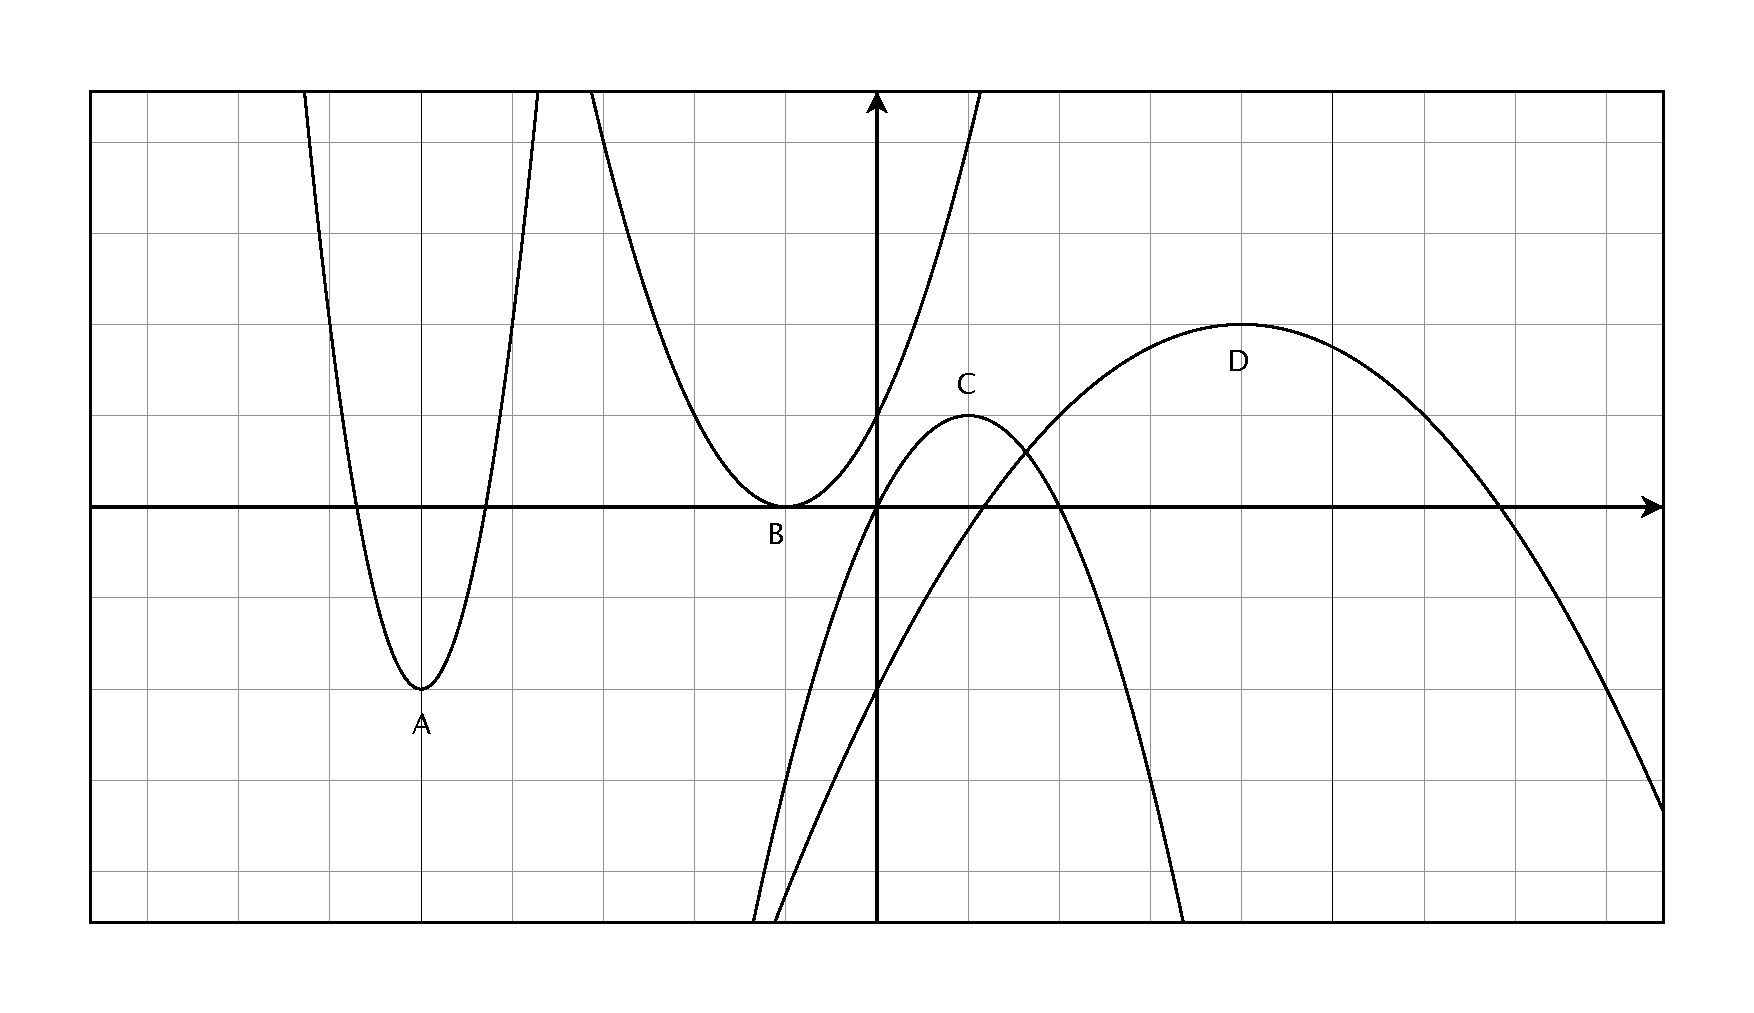
\includegraphics[scale=.3]{problem_7.eps}
%   \caption*{Problem 7}
% \end{figure}

% \begin{tabular}{cc}
% \toprule
% period & amplitude \\
% \midrule
%   $\pi$ & $2$ \\
% \bottomrule
% \end{tabular}

\title{Math 142 Notes \\ Section 6.1}

\date{October 16, 2013}

\begin{document}

  \maketitle
  \tableofcontents

  \section{Angles}

  Degrees may have came from the approximate number of days in a year, 6 times 60 from Babylonians.

  Radians is either:
  \begin{itemize*}
    \item arc length around unit circle
    \item length around any circle divided by the radius
  \end{itemize*}

  conversions:
  \begin{itemize*}
    \item degrees to radians: multiply by $\sfrac{2 \pi}{360 \dg}$
    \item radians to degrees: multiply by $\sfrac{360 \dg}{2 \pi}$
  \end{itemize*}

  examples: $30\dg$, $90\dg$, $\sfrac{\pi}{3}$, etc.

  \section{Reference Angle}
  \begin{itemize*}
    \item like reference number from chapter 5
    \item angle between line and shortest route to x-axis
  \end{itemize*}

  \begin{tabular}[H]{lr}
    \toprule
    angle                & reference angle \\
    \midrule
    $45 \dg$             & $45 \dg$ \\
    $150 \dg$            & $30 \dg$ \\
    $370 \dg$            & $10 \dg$ \\
    $\sfrac{3 \pi}{4}$   & $\sfrac{\pi}{4}$ \\
    $\sfrac{23 \pi}{11}$ & $\sfrac{\pi}{11}$ \\
    $31 \pi$             & $\pi$ \\
    \bottomrule
  \end{tabular}

  \section{Coterminal}
  Angles with the same ending line are ``coterminal.''

  \begin{tabular}[H]{lr}
    \toprule
    $45 \dg$             & $-315 \dg$ \\
    $\sfrac{3 \pi}{4}$   & $\sfrac{11 \pi}{4}$ \\
    $- \sfrac{\pi}{4}$   & $\sfrac{7 \pi}{4}$ \\
    \bottomrule
  \end{tabular}

  \section{Arc Length}

  \begin{itemize*}
    \item find angle in radians
    \item multiply by radius
  \end{itemize*}

  \begin{enumerate}
    \item $\theta = \sfrac{\pi}{5}$, $r = 3$
    \item $\theta = 135 \dg$, $r = 8$
  \end{enumerate}

  \section{Angular Velocity}

  \subsection{Definition}
  \begin{itemize*}
    \item linear velocity: $v = \sfrac{\Delta d}{\Delta t}$
    \item angular velocity: $v = \sfrac{\Delta \theta}{\Delta t}$
  \end{itemize*}

  \subsection{Examples}

\end{document}
